\documentclass[11pt]{article}

% ====================================================
% ====================================================
% USEPACKAGES AND IMPORTS
% ====================================================
% ====================================================

\usepackage[T1]{fontenc}
\usepackage[utf8]{inputenc}
\usepackage[english]{babel}

\usepackage{fancyhdr}

% definitions
% ====================================================
\let\titleoriginal\title
\renewcommand{\title}[1]{
	\titleoriginal{#1}
	\newcommand{\thetitle}{#1}
}

\setlength{\parskip}{\baselineskip}%
\setlength{\parindent}{0pt}%

% header and footer
\pagestyle{fancy}
\fancyhf{}
\lhead{Applied Machine Learning Fundamentals}
\rhead{\thetitle}
\cfoot{\thepage}

% ====================================================
% ====================================================
% PRESENTATION DATA
% ====================================================
% ====================================================

\title[Decision Trees and Ensembles]{*** Applied Machine Learning Fundamentals *** Decision Trees and Ensembles}
\institute[SAP\,SE]{SAP\,SE / DHBW Mannheim}
\author{Daniel Wehner, M.Sc.}
\date{Winter term 2020/2021}
\prefix{DT}

% ====================================================
% ====================================================
% BEGIN OF DOCUMENT
% ====================================================
% ====================================================

\begin{document}

% Title frame
%______________________________________________________________________
\maketitlepage


% Lecture Overview
%______________________________________________________________________
\begin{frame}{Lecture Overview}{}
	\makeoverview{6}
\end{frame}


% Agenda
%______________________________________________________________________
\begin{frame}{Agenda for this Unit}
	\begin{multicols}{2}
		\tableofcontents
	\end{multicols}
\end{frame}


% Section: Introduction
%______________________________________________________________________
\section{Introduction}
\makedivider{Introduction}

% What we want...
\begin{frame}{What we want...}{}
	\divideTwo{0.49}{
		\vspace*{4mm}
		\begin{table}
	\scalebox{0.6}{
	\begin{tabular}{| c | c | c | c | c |}
		\hline
		\highlight{A}	&
		\highlight{F} 	&
		\highlight{S} 	&
		\highlight{N} 	&
		\highlight{H}		\\ \hline\hline
		0	&	1	&	0	&	1	&	1	\\ \hline
		1	&	0	&	0	&	0	&	0	\\ \hline
		1	&	0	&	1	&	0	&	1	\\ \hline
		1	&	1	&	1	&	1	&	0	\\ \hline
		0	&	0	&	1	&	1	&	0	\\ \hline
		0	&	0	&	0	&	1	&	1	\\ \hline
		1	&	0	&	0	&	0	&	0	\\ \hline
		0	&	1	&	0	&	1	&	1	\\ \hline
		1	&	1	&	0	&	0	&	0	\\ \hline
		1	&	0	&	1	&	0	&	1	\\ \hline
		1	&	1	&	1	&	1	&	1	\\ \hline
		1	&	1	&	0	&	1	&	0	\\ \hline
		1	&	0	&	1	&	0	&	0	\\ \hline
		0	&	1	&	0	&	0	&	1	\\ \hline
		1	&	0	&	0	&	1	&	1	\\ \hline
		1	&	1	&	1	&	0	&	0	\\ \hline
	\end{tabular}}
\end{table}
	}{0.49}{
		\input{08_decision_trees/01_tikz/tree}
	}
\end{frame}


% What are Decision Trees?
\begin{frame}{What are Decision Trees?}{}
	\begin{itemize}
		\item Decision trees are induced in a \textbf{supervised} fashion
		\item Originally invented by \textit{Ross Quinlan} (1986)
		\item Decision trees are grown \textbf{recursively} $\rightarrow$ \textit{'divide-and-conquer'}
		\item A decision tree consists of:

		\begin{tabbing}
			\hspace*{2.5cm}\= \kill
			\textbf{Nodes}	\>	Each node corresponds to an attribute test 	\\
			\textbf{Edges}	\>	One edge per possible test outcome			\\
			\textbf{Leaves}	\>	Class label to predict
		\end{tabbing}
	\end{itemize}
\end{frame}


% Classifying new Instances
\begin{frame}{Classifying new Instances}{}
	\divideTwo{0.49}{
		\begin{itemize}
			\item Suppose we get a new instance:
			
			\footnotesize
			\begin{tabbing}
				\hspace*{2.5cm}\= \kill
				\texttt{Outlook}			\>	rainy		\\
				\texttt{Temperature} 		\>	mild	 	\\
				\texttt{Humidity}			\>	normal	\\
				\texttt{Wind}			\>	strong
			\end{tabbing}
			\normalsize

			\item \textbf{What is its class?}
			\item Answer: \textbf{No}
		\end{itemize}
	}{0.49}{
		\input{08_decision_trees/01_tikz/tree}
	}
\end{frame}


% Another Decision Tree...
\begin{frame}{Another Decision Tree...}{}
	\bubble{1}{11}{\footnotesize Is this one better?}
	\vspace*{-2mm}
	% Set the overall layout of the tree
\tikzstyle{level 1}=[level distance=2cm,sibling distance=6cm]
\tikzstyle{level 2}=[level distance=2.5cm,sibling distance=2cm]
\tikzstyle{level 3}=[level distance=2.5cm,sibling distance=1.5cm]

% Define styles for bags and leafs
\tikzstyle{bag}=[rectangle,draw=black,text width=4em,text centered]
\tikzstyle{end}=[circle,draw=black,minimum width=3pt,fill,inner sep=0pt]

\begin{figure}
	\centering
	\begin{tikzpicture}[
		scale=0.6,
		every node/.style={scale=0.5},
		sloped
	]
		\node[bag]{\highlight{Temp.}}
    		child{
     	   		node[bag]{\highlight{Outlook}}        
            			child{
                			node[end, label=below:{\textbf{\underline{No}}}]{}
                			edge from parent
                			node[above]{\textit{sunny}}
            			}
            			child{
                			node[end, label=below:{\textbf{\textcolor{red}{\underline{?}}}}]{}
               			edge from parent
                			node[above]{\textit{rain}}
            			}
				child{
                			node[end, label=below:{\textbf{\underline{Yes}}}]{}
               			edge from parent
                			node[above]{\textit{overcast}}
            			}
            			edge from parent 
            			node[above]{\textit{hot}}
    		}
		child{
        		node[bag]{\highlight{Outlook}}        
        		child {
                		node[bag]{\highlight{Humid.}}
                		child{
                			node[end, label=below:{\textbf{\underline{No}}}]{}
                			edge from parent
                			node[above]{\textit{high}}
                		}
				child{
                			node[end, label=below:{\textbf{\underline{Yes}}}]{}
                			edge from parent
                			node[above]{\textit{normal}}
                		}
				child[missing]{}
                		edge from parent
                		node[above]{\textit{sunny}}
            		}
            		child{
                		node[bag]{\highlight{Humid.}}
				child[missing]{}
				child{
					node[bag]{\highlight{Wind}}
					child{
						node[end, label=below:{\textbf{\underline{No}}}]{}
                				edge from parent
                				node[above]{\textit{strong}}
					}
					child{
						node[end, label=below:{\textbf{\underline{Yes}}}]{}
                				edge from parent
                				node[above]{\textit{weak}}
					}
					edge from parent
                			node[above]{\textit{high}}
				}
				child{
					node[end, label=below:{\textbf{\underline{Yes}}}]{}
                			edge from parent
                			node[above]{\textit{normal}}
				}
                		edge from parent
                		node[above]{\textit{rainy}}
            		}
			child{
                		node[end, label=below:{\textbf{\underline{Yes}}}]{}
                		edge from parent
                		node[above]{\textit{overcast}}
            		}
        		edge from parent         
            		node[above]{\textit{mild}}
		}
    		child{
        		node[bag]{\highlight{Outlook}}        
        		child {
                		node[end, label=below:{\textbf{\underline{Yes}}}]{}
                		edge from parent
                		node[above]{\textit{sunny}}
            		}
            		child{
                		node[bag]{\highlight{Humid.}}
                		child{
                			node[end, label=below:{\textbf{\textcolor{red}{\underline{?}}}}]{}
                			edge from parent
                			node[above]{\textit{high}}
                		}
				child{
                			node[bag]{\highlight{Wind}}
					child{
                				node[end, label=below:{\textbf{\underline{No}}}]{}
                				edge from parent
                				node[above]{\textit{strong}}
                			}
					child{
                				node[end, label=below:{\textbf{\underline{Yes}}}]{}
                				edge from parent
                				node[above]{\textit{weak}}
                			}
                			edge from parent
                			node[above]{\textit{normal}}
                		}
                		edge from parent
                		node[above]{\textit{rainy}}
            		}
			child{
                		node[end, label=below:{\textbf{\underline{Yes}}}]{}
                		edge from parent
                		node[above]{\textit{overcast}}
            		}
        		edge from parent         
            		node[above]{\textit{cool}}
		};
	\end{tikzpicture}
\end{figure}
\end{frame}


% Section: Iterative Dichotomizer (ID3)
%______________________________________________________________________
\section{Iterative Dichotomizer (ID3)}
\makedivider{Iterative Dichotomizer (ID3)}

% Subsection: Inductive Bias
% --------------------------------------------------------------------------------------------------------
\subsection{Inductive Bias}

% Inductive Bias of Decision Trees
\begin{frame}{Inductive Bias of Decision Trees}{}\important
	\divideTwo{0.75}{
		\begin{itemize}
			\item Complex models tend to \textbf{overfit} the data and \textbf{do not generalize well}
			\item Small decision trees are preferred
			\vspace*{4mm}
			\begin{boxBlueNoFrame}
				\textbf{Occam's razor}: \\
				\footnotesize \textbf{`More things should not be used than are necessary.'}
			\end{boxBlueNoFrame}
			\vspace*{2mm}
			\item \highlight{Prefer the simplest hypothesis that fits the data!}
		\end{itemize}
	}{0.20}{
		\begin{figure}
			\centering
			\fbox{\includegraphics[scale=0.2]{08_decision_trees/02_img/william_of_ockham}}
		\end{figure}
	}
\end{frame}


% The Root of all Evil... Which Attribute to choose?
\begin{frame}{The Root of all Evil... Which Attribute to choose?}{}
	\divideTwo{0.49}{
		\input{08_decision_trees/01_tikz/attribute_split_outlook}
		\vspace*{0.25mm}	
	}{0.49}{
		% Set the overall layout of the tree
\tikzstyle{level 1}=[level distance=3.5cm, sibling distance=2cm]
\tikzstyle{level 2}=[level distance=3.5cm, sibling distance=2cm]

% Define styles for bags and leafs
\tikzstyle{bag} = [rectangle, draw=black, text width=4em, text centered]
\tikzstyle{end} = [circle, draw=black, minimum width=3pt, fill, inner sep=0pt]

\begin{figure}
	\centering
	\begin{tikzpicture}[
		scale=0.6,
		every node/.style={scale=0.5},
		sloped
	]
		\node[bag]{\highlight{Temp.}}
		child{
			node[bag,align=center]{Yes Yes\\No No}
			edge from parent
			node[above]{\textit{hot}}
		}
    		child{
			node[bag,align=center]{Yes Yes\\Yes Yes\\No No}
			edge from parent
			node[above]{\textit{mild}}
		}
		child{
			node[bag,align=center]{Yes Yes\\Yes No}
			edge from parent
			node[above]{\textit{cool}}
		};
	\end{tikzpicture}
\end{figure}
		\vspace*{0.25mm}	
	}

	\divideTwo{0.49}{
		\input{08_decision_trees/01_tikz/attribute_split_wind}
	}{0.49}{
		\input{08_decision_trees/01_tikz/attribute_split_humidity}
	}
\end{frame}


% Subsection: Entropy and Information Gain
% --------------------------------------------------------------------------------------------------------
\subsection{Entropy and Information Gain}

% Finding a proper Attribute
\begin{frame}{Finding a proper Attribute}{}
	\divideTwo{0.79}{
		\begin{itemize}
			\item Simple and small trees are preferred
			\begin{itemize}
				\item Data in successor node should be \textbf{as pure as possible}
				\item I.\,e. nodes containing one class only are preferable
			\end{itemize}
			\item \textbf{Question:} How can we express this thought as a mathematical formula?
			\item \textbf{Answer:}
			\begin{itemize}
				\item \highlight{Entropy} (\textit{Claude E. Shannon})
				\item Originates in the field of \textbf{information theory}
			\end{itemize}
		\end{itemize}
	}{0.19}{
		\fbox{\includegraphics[scale=0.3]{08_decision_trees/02_img/claude_shannon}}
	}
\end{frame}


% Measure of Impurity: Entropy
\begin{frame}{Measure of Impurity: Entropy}{}
	\begin{itemize}
		\item Entropy is a measure of chaos in the data (measured in bits)
		\item \textbf{Example:} Consider two classes $A$ and $B$ ($\mathcal{C} = \{ A, B \}$)
	
		\footnotesize
		\begin{tabbing}
			\hspace*{5cm}\=\hspace*{1.5cm}\= \kill
			$E(\{ \bm{A}, \bm{A}, \bm{A}, \bm{A}, \bm{A}, \bm{A}, \bm{A}, \bm{A} \})$
				\>	$\rightarrow$ 0		\>	$Bits$	\\
			$E(\{ \bm{A}, \bm{A}, \bm{A}, \bm{A}, \bm{A}, \bm{A}, B, B \})$
				\>	$\rightarrow$ 0.81 	\>	$Bits$	\\
			$E(\{ \bm{A}, \bm{A}, \bm{A}, \bm{A}, B, B, B, B \})$
				\>	$\rightarrow$ 1		\>	$Bit$		\\
			$E(\{ \bm{A}, \bm{A}, B, B, B, B, B, B \})$
				\>	$\rightarrow$ 0.81 	\>	$Bits$	\\
			$E(\{ B, B, B, B, B, B, B, B \})$	
				\>	$\rightarrow$ 0		\>	$Bits$
		\end{tabbing}
		\normalsize
	\end{itemize}
	
	\begin{boxBlueNoFrame}
		\footnotesize
		\highlight{If both classes are equally distributed, the entropy function $E$ reaches its maximum.
		Pure data sets have minimal entropy}.
	\end{boxBlueNoFrame}
\end{frame}


% Measure of Impurity: Entropy (Ctd.)
\begin{frame}{Measure of Impurity: Entropy (Ctd.)}{}
	\begin{figure}
	\centering
	\begin{tikzpicture}
    
    		\begin{axis}[
			scale=0.7,
			xlabel={Relative frequency of class $A$ ($p_A$)},
			ylabel={Entropy $E(\mathcal{D})$},
			grid=both,
    			grid style={line width=.1pt, draw=gray!10},
			minor tick num=2,
    			major grid style={line width=.2pt,draw=gray!80},
			minor grid style={line width=.2pt,draw=gray!30},
  			x=10cm,
  			y=5.5cm
		]

			\pgfplotstableread{08_decision_trees/05_data/data_entropy.txt} \datatable
			\addplot[myblue1,no marks,ultra thick,smooth] table[x=x,y=y] from \datatable;

			\node[fill=myblue1] at (axis cs:0.5,0.45) {\footnotesize $\textcolor{white}{E(\mathcal{D}) =
				-\sum_{c \in \mathcal{C}} p_c \cdot \log_2 p_c}$};
		
		\end{axis}
	\end{tikzpicture}
\end{figure}
\end{frame}


% Measure of Impurity: Entropy (Ctd.)
\begin{frame}{Measure of Impurity: Entropy (Ctd.)}{}\important
	\vspace*{2mm}
	\begin{boxBlueNoFrame}
		\highlight{Entropy formula:}
		\begin{equation}
			E(\mathcal{D}) = -\sum_{c \in \mathcal{C}} p_c \cdot \log_2 p_c
		\end{equation}
	\end{boxBlueNoFrame}

	\begin{itemize}
		\item $p_c$ denotes the relative frequency of class $c \in \mathcal{C}$	
		\item \textbf{Weather data:}
		\begin{align*}
			\mathcal{C} &= \{ yes, no \} \qquad \text{i.\,e.} \qquad
				p_{yes} = \nicefrac{9}{14} \quad \text{and} \quad p_{no} = \nicefrac{5}{14} \\[3mm]
			E(\mathcal{D})
				&= -\sum_{c \in \mathcal{C}} p_c \cdot \log_2 p_c
	       		   	= - (\nicefrac{9}{14} \cdot \log_2 \nicefrac{9}{14} + \nicefrac{5}{14} \cdot \log_2 \nicefrac{5}{14})
				= \boldsymbol{0.9403}
		\end{align*}
	\end{itemize}
\end{frame}


% Quality of the Split: Average Entropy
\begin{frame}{Quality of the Split: Average Entropy}{}
	\begin{itemize}
		\item We still don't know which attribute to use for the split
		\item Calculate the entropy after each potential split
		\item \highlight{Average Entropy} after splitting by attribute \texttt{A}:
		\begin{equation}
			E(\mathcal{D}, \texttt{A})
				= \sum_{v \in \text{dom}(\texttt{A})}
					\frac{\vert \mathcal{D}_{\texttt{A}=v} \vert}{\vert \mathcal{D} \vert} \cdot E(\mathcal{D}_{\texttt{A}=v})
		\end{equation}
		\item Legend:
		\footnotesize
		\begin{tabbing}
			\hspace*{2.5cm}\= \kill
			\texttt{A}							\>	Attribute												\\
			$\text{dom}(\texttt{A})$				\>	Possible values attribute \texttt{A} can take (domain of \texttt{A})	\\
			$\vert \mathcal{D}_{\texttt{A}=v} \vert$	\>	Number of examples satisfying $\texttt{A} = v$
		\end{tabbing}
		\normalsize
	\end{itemize}
\end{frame}


% Quality of the Split: Average Entropy (Ctd.)
\begin{frame}{Quality of the Split: Average Entropy (Ctd.)}{}
	\textbf{Example:} Attribute \texttt{Outlook}
	\begin{alignat*}{2}
		E(\mathcal{D}, \texttt{Outlook})
			&= \sum_{v \in \text{dom}(\texttt{Outlook})}
				\frac{\vert \mathcal{D}_{\texttt{Outlook} = v} \vert}{\vert \mathcal{D} \vert} \cdot E(\mathcal{D}_{\texttt{Outlook} = v}) 	\\[2mm]
			&= \nicefrac{5}{14} \cdot 0.9710 + \nicefrac{5}{14} \cdot 0.9710 + \nicefrac{4}{14} \cdot 0
			&&= \bm{0.6936}																				\\[2mm]
																										\hline
																										\\[-3mm]
		E(\mathcal{D}_{\texttt{Outlook}=sunny})
			&= -(\nicefrac{2}{5} \cdot \log_2 (\nicefrac{2}{5}) + \nicefrac{3}{5} \cdot \log_2 (\nicefrac{3}{5}))
			&&= 0.9710																					\\[2mm]
		E(\mathcal{D}_{\texttt{Outlook}=rainy})
			&= -(\nicefrac{3}{5} \cdot \log_2 (\nicefrac{3}{5}) + \nicefrac{2}{5} \cdot \log_2 (\nicefrac{2}{5}))
			&&= 0.9710																					\\[2mm]
		E(\mathcal{D}_{\texttt{Outlook}=overcast})
			&= -(\nicefrac{4}{4} \cdot \log_2 (\nicefrac{4}{4}) + \nicefrac{0}{4} \cdot \log_2 (\nicefrac{0}{4}))
			&&= 0
	\end{alignat*}
\end{frame}


% Information Gain
\begin{frame}{Information Gain}{}
	\begin{itemize}
		\item We have calculated the entropy before and after the split
		\item The difference of both is called the \highlight{information gain (IG)}
		\item Select the attribute with the highest IG
		\vspace*{2mm}
		\begin{table}[h]
	\scalebox{0.8}{
		\begin{tabular}{| l | c | c | c |}
			\hline
			\textbf{Attribute}	& $\bm{E_{before}}$ & $\bm{E_{after}}$ & $\bm{IG}$ \\
			\hline\hline
			\rowcolor{myblue1!70}
			\texttt{Outlook}			& 0.9403 & 0.6936 & 0.2464 	\\ \hline
			\texttt{Temperature}		& 0.9403 & 0.9111 & 0.0292 	\\ \hline
			\texttt{Humidity}			& 0.9403 & 0.7885 & 0.1518 	\\ \hline
			\texttt{Wind}			& 0.9403 & 0.8922 & 0.0481	\\ \hline
		\end{tabular}
	}
\end{table}
		\vspace*{2mm}
		\item Attribute \texttt{Outlook} maximizes IG
		\item After the split: Remove attribute \texttt{Outlook}
	\end{itemize}
\end{frame}


% Training Data after the Split by Attribute \texttt{Outlook}
\begin{frame}{Training Data after the Split by Attribute \texttt{Outlook}}{}
	\divideTwo{0.49}{
		\vspace*{5mm}
		\begin{table}[h]

	\scalebox{0.6}{
		\begin{tabular}{| c | c | c | c | c |}
			\hline
			\st{Outlook}				&
			\highlight{Temperature} 		&
			\highlight{Humidity} 			&
			\highlight{Wind} 			&
			\highlight{PlayGolf}			\\ \hline\hline
			\rowcolor{gray!30}
			\st{sunny} 		& hot 		& high 		& weak 		& no 		\\ \hline
			\rowcolor{gray!30}
			\st{sunny} 		& hot 		& high 		& strong 		& no 		\\ \hline
			\rowcolor{gray!30}
			\st{sunny} 		& mild 		& high 		& weak 		& no 		\\ \hline
			\rowcolor{gray!30}
			\st{sunny} 		& cool 		& normal 		& weak 		& yes 	\\ \hline
			\rowcolor{gray!30}
			\st{sunny} 		& mild 		& normal 		& strong 		& yes 	\\ \hline\hline
			\rowcolor{gray!60}
			\st{rainy} 		& mild 		& high 		& weak 		& yes 	\\ \hline
			\rowcolor{gray!60}
			\st{rainy} 		& cool 		& normal 		& weak 		& yes 	\\ \hline
			\rowcolor{gray!60}
			\st{rainy} 		& cool 		& normal 		& strong 		& no 		\\ \hline
			\rowcolor{gray!60}
			\st{rainy} 		& mild 		& normal 		& weak 		& yes	\\ \hline
			\rowcolor{gray!60}
			\st{rainy} 		& mild 		& high 		& strong 		& no 		\\ \hline\hline
			\rowcolor{gray!90}
			\st{overcast} 	& cool 		& normal 		& strong 		& yes 	\\ \hline
			\rowcolor{gray!90}
			\st{overcast} 	& hot 		& high 		& weak 		& yes 	\\ \hline
			\rowcolor{gray!90}
			\st{overcast} 	& mild 		& high 		& strong 		& yes 	\\ \hline
			\rowcolor{gray!90}
			\st{overcast} 	& hot 		& normal 		& weak 		& yes 	\\ \hline
		\end{tabular}
	}

\end{table}
	}{0.49}{
		\begin{itemize}
			\item Data set $\mathcal{D}$ after the split
			\item We obtain three subsets (one per attribute value)
			\item Attribute \texttt{Outlook} is removed
		\end{itemize}
	}
\end{frame}


% Subsection: ID3 Algorithm
% --------------------------------------------------------------------------------------------------------
\subsection{ID3 Algorithm}

% How to proceed?
\begin{frame}{How to proceed?}{}\important
	\begin{itemize}
		\item The algorithm is recursively applied to the resulting subsets
		\begin{enumerate}
			\item Calculate entropy (before and after the split)
			\item Calculate information gain for each attribute 
			\item Choose the attribute with max. information gain for the split
			\item In the current branch: Do not consider the attribute any more
			\item \textbf{Recursion} $\bm{\circlearrowleft}$ (\texttt{Go to 1})
		\end{enumerate}
		\item Recursion stops as soon as the subset is pure
		\item In the example above the subset $\mathcal{D}_{\texttt{Outlook}=overcast}$ is already pure
		\item This algorithm is referred to as \highlight{ID3 (Iterative Dichotomizer)}
	\end{itemize}
\end{frame}


% Step by Step: Construction of the Tree
\begin{frame}{Step by Step: Construction of the Tree}{}
	{
% Set the overall layout of the tree
\tikzstyle{level 1}=[level distance=2.5cm,sibling distance=3cm]
\tikzstyle{level 2}=[level distance=2.5cm,sibling distance=3cm]

% Define styles for bags and leafs
\tikzstyle{bag}=[rectangle,draw=black,text width=4em,text centered]
\tikzstyle{end}=[circle,draw=black,minimum width=3pt,fill,inner sep=0pt]

\begin{figure}
	\centering
	\begin{tikzpicture}[
		sloped
	]
		\node[bag]{\highlighttt{Outlook}}
    		child {
      		  	node[bag]{?}
     	  	     	edge from parent 
 	           	node[above]{\textit{sunny}}
    		}
		child {
			node[bag]{?}
			edge from parent
			node[above]{\textit{overcast}}
		}
    		child {
        			node[bag]{?}
        			edge from parent         
	       	     	node[above]{\textit{rainy}}
		};
	\end{tikzpicture}
\end{figure}}
\end{frame}


% Step by Step: Construction of the Tree (Ctd.)
\begin{frame}{Step by Step: Construction of the Tree (Ctd.)}{}
	\divideTwo{0.49}{
		{
% Set the overall layout of the tree
\tikzstyle{level 1}=[level distance=2.5cm,sibling distance=3cm]
\tikzstyle{level 2}=[level distance=2.5cm,sibling distance=3cm]

% Define styles for bags and leafs
\tikzstyle{bag}=[rectangle,draw=black,text width=4em,text centered]
\tikzstyle{end}=[circle,draw=black,minimum width=3pt,fill,inner sep=0pt]

\begin{figure}
	\centering
	\begin{tikzpicture}[
		scale=0.5,
		every node/.style={scale=0.5},
		sloped
	]
		\node[bag]{\highlight{Outlook}}
    		child {
     	 	  	node[bag]{\highlight{Temp.}}
			child {
				node[bag,align=center]{No No}
                			edge from parent
                			node[above]{\textit{hot}}
			}
			child {
				node[bag,align=center]{Yes No}
                			edge from parent
                			node[above]{\textit{mild}}
			}
			child {
				node[bag,align=center]{Yes}
                			edge from parent
                			node[above]{\textit{cool}}
			}
            		edge from parent 
            		node[above]{\textit{sunny}}
    		}
		child {
			node[bag]{?}
			edge from parent
			node[above]{\textit{overcast}}
		}
    		child {
        			node[bag]{?}
        			edge from parent         
            		node[above]{\textit{rainy}}
		};
	\end{tikzpicture}
\end{figure}}
		\vspace*{0.25mm}
	}{0.49}{
		\vspace*{1mm}
		{
% Set the overall layout of the tree
\tikzstyle{level 1}=[level distance=2.5cm,sibling distance=3cm]
\tikzstyle{level 2}=[level distance=2.5cm,sibling distance=3cm]

% Define styles for bags and leafs
\tikzstyle{bag}=[rectangle,draw=black,text width=4em,text centered]
\tikzstyle{end}=[circle,draw=black,minimum width=3pt,fill,inner sep=0pt]

\begin{figure}
	\centering
	\begin{tikzpicture}[
		scale=0.45,
		every node/.style={scale=0.5},
		sloped
	]
		\node[bag]{\highlighttt{Outlook}}
    		child {
     	   		node[bag]{\highlighttt{Humid.}}
			child {
				node[bag,align=center]{No No\\No}
     	     		      	edge from parent
     		           	node[above]{\textit{high}}
			}
			child {
				node[bag,align=center]{Yes Yes}
                			edge from parent
                			node[above]{\textit{normal}}
			}
            		edge from parent 
            		node[above]{\textit{sunny}}
    		}
		child {
			node[bag]{?}
			edge from parent
			node[above]{\textit{overcast}}
		}
    		child {
        			node[bag]{?}
        			edge from parent         
            		node[above]{\textit{rainy}}
		};
	\end{tikzpicture}
\end{figure}}
		\vspace*{0.25mm}
	}
	
	\divideTwo{0.49}{
		\input{08_decision_trees/01_tikz/tree_construction_2_alternative_3}
	}{0.49}{
		\begin{itemize}
			\item $IG(\texttt{Temperature}) = 0.571$
			\item $IG(\texttt{Humidity}) = \textbf{0.971}$
			\item $IG(\texttt{Wind}) = 0.020$
		\end{itemize}
	}
\end{frame}


% Step by Step: Construction of the Tree (Ctd.)
\begin{frame}{Step by Step: Construction of the Tree (Ctd.)}{}
	\input{08_decision_trees/01_tikz/tree_construction_2_result}
\end{frame}


% Step by Step: Construction of the Tree (Ctd.)
\begin{frame}{Step by Step: Construction of the Tree (Ctd.)}{}
	\input{08_decision_trees/01_tikz/tree_construction_3_result}
\end{frame}


% Step by Step: Construction of the Tree (Ctd.)
\begin{frame}{Step by Step: Construction of the Tree (Ctd.)}{}
	{
% Set the overall layout of the tree
\tikzstyle{level 1}=[level distance=2.5cm, sibling distance=3cm]
\tikzstyle{level 2}=[level distance=2.5cm, sibling distance=3cm]

% Define styles for bags and leafs
\tikzstyle{bag}=[rectangle,draw=black,text width=4em,text centered]
\tikzstyle{end}=[circle,draw=black,minimum width=3pt,fill,inner sep=0pt]

\begin{figure}
	\centering
	\begin{tikzpicture}[
		scale=0.9,
		every node/.style={scale=0.9},
		sloped
	]
		\node[bag]{\highlight{Outlook}}
    		child {
        			node[bag]{\highlight{Humid.}}        
        			child {
            	    		node[end,label=below:{\textbf{\underline{No}}}]{}
            	    		edge from parent
            		    	node[above]{\textit{high}}
            		}
            		child {
                			node[end,label=below:{\textbf{\underline{Yes}}}]{}
                			edge from parent
                			node[above]{\textit{normal}}
            		}
        			edge from parent         
            		node[above]{\textit{sunny}}
		}
		child {
			node[end,label=below:{\textbf{\underline{Yes}}}]{}
			edge from parent
			node[above]{\textit{overcast}}
		}
		child {
        			node[bag]{\highlight{Wind}}        
            		child {
              	  		node[end,label=below:{\textbf{\underline{No}}}]{}
                			edge from parent
                			node[above]{\textit{strong}}
            		}
            		child {
           	     		node[end,label=below:{\textbf{\underline{Yes}}}]{}
               			edge from parent
                			node[above]{\textit{weak}}
            		}
            		edge from parent 
            		node[above]{\textit{rainy}}
    		};
	\end{tikzpicture}
\end{figure}}
\end{frame}


% ID3 Algorithm
\begin{frame}[plain]{}{}
	\begin{algorithm}[H]
	\setstretch{1.0}
	\DontPrintSemicolon
	\footnotesize
	\KwIn{Training set $\mathcal{D}$, Attribute list $Attr\_List$}
	Create a node $N$\;
	\If{all tuples in $\mathcal{D}$ have class $c$}{
		\Return{$N$ as leaf node labeled with class $c$}
	}
	\If{$\vert Attr\_List \vert = 0$}{
		\Return{$N$ as leaf node labeled with majority class in $\mathcal{D}$}
	}
	Find best split attribute $\texttt{A}^*$ and label node $N$ with $\texttt{A}^*$\;
	$Attr\_List \longleftarrow Attr\_List \backslash \{ \texttt{A}^* \}$\;
	\ForAll{$v \in \text{dom}(\texttt{A}^*)$}{
		Let $\mathcal{D}_{\texttt{A}^*=v}$ be the set of tuples in $\mathcal{D}$ that satisfy $\texttt{A}^* = v$\;
		\If{$\vert \mathcal{D}_{\texttt{A}^*=v} \vert = 0$}{
			Attach leaf labeled with majority class in $\mathcal{D}$ to node $N$\;
		}
		\Else{
			Attach node returned by $ID3(\mathcal{D}_{\texttt{A}^*=v}, Attr\_List)$\;
		}
	}
	
	\Return{$N$}
 	\caption{ID3 Algorithm (Iterative Dichotomizer)}
\end{algorithm}
\end{frame}


% Section: Extensions and Variants
%______________________________________________________________________
\section{Extensions and Variants}
\makedivider{Extensions and Variants}

% Subsection: Other Measures of Impurity
% --------------------------------------------------------------------------------------------------------
\subsection{Other Measures of Impurity}

% An Alternative to Information Gain: Gini Index
\begin{frame}{An Alternative to Information Gain: Gini Index}{}
	\begin{boxBlueNoFrame}
		\highlight{Gini index:}
		\begin{equation}
			Gini(\mathcal{D})
				= \sum_{c \in \mathcal{C}} p_c \cdot (1 - p_c)
				= 1 -  \sum_{c \in \mathcal{C}} p_c^2
		\end{equation}
	\end{boxBlueNoFrame}
	\begin{itemize}
		\item Used e.\,g. in \highlight{CART (Classification and Regression Trees)}
		\item \textbf{Gini gain} could be defined analogously to IG \\
			{\footnotesize \textit{(usually not done)}}
	\end{itemize}
\end{frame}


% Why not use the Error as a splitting Criterion?
\begin{frame}{Why not use the Error as a splitting Criterion?}{}\optional
	\begin{itemize}
		\item The bias towards pure leaves is \textbf{not strong enough}
		\item \textbf{Example:}
	\end{itemize}
	
	\divideTwo{0.49}{
		\vspace*{2mm}
		\begin{figure}
	\centering
	\begin{tikzpicture}[
		scale=0.5
	]
	
		\draw[fill=lightgray] (0,0) rectangle (3,3);
		\draw[fill=lightgray] (0,3) rectangle (3,6);
		\draw[fill=lightgray] (3,3) rectangle (6,6);
		\draw[fill=myblue1!70] (3,0) rectangle (6,3);
		\draw[very thick] (0,0) rectangle (6,6);

		\node[rotate=90] at (-1,3) {\textbf{Split 1}};
		\node at (3,-1) {\textbf{Split 2}};

		\node at (1.5,1.5) {60 of A};
		\node at (1.5,4.5) {40 of A};
		\node at (4.5,4.5) {60 of A};
		\node at (4.5,1.5) {40 of B};
		
	\end{tikzpicture}
\end{figure}
	}{0.49}{
		Error without splitting: \\
		\textbf{20\,\%} \\ \vspace*{-3mm}
		
		Error after splitting: \\
		\textbf{20\,\%} \\ \vspace*{-3mm}
		
		\footnotesize
		\highlight{Both splits don't improve the error. \\
		But together they give a perfect split!}
	}
\end{frame}


% Summary: Impurity Measures
\begin{frame}{Summary: Impurity Measures}{}
	\begin{figure}
\centering
\begin{tikzpicture}
    
    \begin{axis}[
		scale=0.7,
		xlabel={Relative frequency of class $A$ ($p_a$)},
		ylabel={Impurity Measures},
		grid=both,
    		grid style={line width=.1pt, draw=gray!10},
		minor tick num=2,
    		major grid style={line width=.2pt,draw=gray!80},
		minor grid style={line width=.2pt,draw=gray!30},
  		x=8cm,
  		y=5.5cm,
		legend pos=outer north east
	]

		\pgfplotstableread{08_decision_trees/05_data/data_impurity_measures_all.txt} \datatable

		\addplot[myblue1,no marks,ultra thick,smooth] table[x=x,y=y1] from \datatable;
		\addlegendentry{Entropy}
		
		\addplot[gray,no marks,ultra thick,smooth] table[x=x,y=y2] from \datatable;
		\addlegendentry{Gini Idx}
	
		\addplot[black,no marks,ultra thick] table[x=x,y=y3] from \datatable;
		\addlegendentry{Error}
		
	\end{axis}

\end{tikzpicture}
\end{figure}
\end{frame}


% Subsection: Highly-branching Attributes
% --------------------------------------------------------------------------------------------------------
\subsection{Highly-branching Attributes}

% Highly-branching Attributes
\begin{frame}{Highly-branching Attributes}{}
	\begin{boxBlueNoFrame}
		\highlight{Attributes with a large number of values are problematic, since the leaves are not
			`backed' with sufficient data examples.}

		\vspace*{4mm}
		\textbf{In extreme cases only one example per node (e.\,g. IDs)}
	\end{boxBlueNoFrame}

	\begin{boxBlueNoFrame}
		This may lead to:
		\begin{itemize}
			\item \textbf{Overfitting} \footnotesize (Selection of attributes which are not optimal for prediction) \normalsize
			\item \textbf{Fragmentation} \footnotesize (Data is fragmented into (too) many small sets) \normalsize
		\end{itemize}
	\end{boxBlueNoFrame}
\end{frame}


% Highly-branching Attributes (Ctd.)
\begin{frame}{Highly-branching Attributes (Ctd.)}{}
	\vspace*{-2mm}
	% Set the overall layout of the tree
\tikzstyle{level 1}=[level distance=2.5cm,sibling distance=2cm]
\tikzstyle{level 2}=[level distance=2.5cm,sibling distance=2cm]

% Define styles for bags and leafs
\tikzstyle{bag}=[rectangle,draw=black,text width=4em,text centered]
\tikzstyle{end}=[circle,draw=black,minimum width=3pt,fill,inner sep=0pt]

\begin{figure}
	\centering
	\begin{tikzpicture}[
		scale=0.9,
		sloped
	]
		\node[bag]{\highlighttt{Day}}
    		child{
     		   	node[end,label=below:{\textbf{\underline{No}}}]{}      
     	       	edge from parent 
      		      	node[above]{\textit{\footnotesize 5 May}}
    		}
		child{
        		node[end,label=below:{\textbf{\underline{No}}}]{}      
            		edge from parent 
            		node[above]{\textit{\footnotesize 6 May}}
    		}
    		child{
        		node[end,label=below:{\textbf{\underline{No}}}]{}      
            		edge from parent 
            		node[above]{\textit{\footnotesize 7 May}}
    		}
		child{
        		node[end,label=below:{\textbf{\underline{Yes}}}]{}      
            		edge from parent 
            		node[above]{\textit{\footnotesize 8 May}}
    		}
    		child{
        		node[end,label=below:{\textbf{...}}]{}      
            		edge from parent 
            		node[above]{\textit{...}}
    		};
	\end{tikzpicture}
\end{figure}
	\vspace*{-5mm}
	\begin{itemize}
		\item Entropy before was $0.9403$, Entropy after split is $0$
		\item IG($\mathcal{D}$, \texttt{Day}) = 0.9403
		\item Attribute \texttt{Day} would be chosen for the split \Highlight{$\Rightarrow$ Bad for prediction $\skull$}
	\end{itemize}
\end{frame}


% Highly-branching Attributes (Ctd.)
\begin{frame}{Highly-branching Attributes (Ctd.)}{}
	\begin{itemize}
		\item Calculate the \highlight{intrinsic information (IntI)}:
		\begin{equation}
			IntI(\mathcal{D}, \texttt{A})
				= -\sum_{v \in \text{dom}(\texttt{A})} \frac{\vert \mathcal{D}_{\texttt{A}=v} \vert}{\vert \mathcal{D} \vert} \cdot
					\log_2 \frac{\vert \mathcal{D}_{\texttt{A}=v} \vert}{\vert \mathcal{D} \vert}
		\end{equation}
		\item Attributes with high $IntI$ are \textbf{less useful} (high fragmentation)
		\item New splitting heuristic \highlight{Gain ratio (GR)}:
		\begin{equation}
			GR(\mathcal{D}, \texttt{A}) = \frac{IG(\mathcal{D}, \texttt{A})}{IntI(\mathcal{D}, \texttt{A})}
		\end{equation}
	\end{itemize}
\end{frame}


% Highly-branching Attributes (Ctd.)
\begin{frame}{Highly-branching Attributes (Ctd.)}{}
	\begin{itemize}
		\item Intrinsic information for attribute \texttt{Day}:
		\begin{equation}
			IntI(\mathcal{D}, \texttt{Day}) = 14 \cdot (-\nicefrac{1}{14} \cdot \log_2 (\nicefrac{1}{14})) = \bm{3.807}
		\end{equation}
		\item Gain ratio for attribute \texttt{Day}:
		\begin{equation}
			GR(\mathcal{D}, \texttt{Day}) = \frac{0.9403}{3.807} = \bm{0.246}
		\end{equation}
	\end{itemize}

	\vspace*{-3mm}
	\begin{boxBlueNoFrame}
		\footnotesize
		In this case the attribute \texttt{Day} would still be chosen.
		Be careful what features to include into the training data set! \highlight{(feature engineering is important!)}
	\end{boxBlueNoFrame}
\end{frame}


% Subsection: Numeric Attributes
% --------------------------------------------------------------------------------------------------------
\subsection{Numeric Attributes}

% Handling numeric Attributes
\begin{frame}{Handling numeric Attributes}{}
	\begin{itemize}
		\item Usually, only \textbf{binary splits} are considered, e.\,g.:
		\begin{itemize}
			\item $\texttt{Temperature} < 48$
			\item $\texttt{CPU} > 24$
			\item \textbf{Not:} $24 \le \texttt{Temperature} \le 31$
		\end{itemize}
		\item To support multiple splits, the attribute is \textbf{not removed} \\
			{\footnotesize \textit{(the same attribute can be used again for another split)}}
		\item \Highlight{Problem:} There is an \textbf{infinite number} of possible splits!
		\item \textbf{Solution:} Discretize range (fixed step size, ...)
		\item \highlight{Splitting on numeric attributes is computationally demanding!}
	\end{itemize}
\end{frame}


% Handling numeric Attributes (Ctd.)
\begin{frame}{Handling numeric Attributes (Ctd.)}{}\important
	\begin{itemize}
		\item Consider the attribute \texttt{Temperature}: \\
			Use \textbf{numerical values} instead of discrete values like \textit{cool}, \textit{mild}, \textit{hot}:
	\end{itemize}
	\vspace*{-3mm}
	\begin{figure}
	\centering
	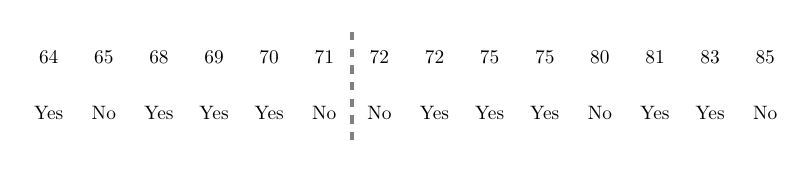
\begin{tikzpicture}[
		scale=0.7,
		every node/.style={scale=0.7}
	]

		\foreach \x/\v/\l in {
			1/64/Yes,2/65/No,3/68/Yes,4/69/Yes,5/70/Yes,6/71/No,7/72/No,
			8/72/Yes,9/75/Yes,10/75/Yes,11/80/No,12/81/Yes,13/83/Yes,14/85/No}{
			\node at (\x, 0) {\highlight{\v}};
			\node at (\x, -1) {\highlight{\l}};
		}

		\draw[gray,dashed,ultra thick] (6.5,-1.5) -- (6.5,0.5);
		
	\end{tikzpicture}
\end{figure}
	\divideTwo{0.49}{
		\begin{itemize}
			\item $\texttt{Temperature} < 71.5$ \\
				{\footnotesize yes: 4 | no: 2}
		\end{itemize}
	}{0.49}{
		\begin{itemize}
			\item $\texttt{Temperature} \ge 71.5$ \\
				{\footnotesize yes: 5 | no: 3}
		\end{itemize}
	}
	\vspace*{2mm}
	\begin{equation*}
			E(\mathcal{D}, \texttt{Temp.})
				= \nicefrac{6}{14} \cdot E(\texttt{Temp.} < 71.5) + \nicefrac{8}{14} \cdot E(\texttt{Temp.} \ge 71.5)
				= \bm{0.939}
		\end{equation*}
\end{frame}


% Handling numeric Attributes (Ctd.)
\begin{frame}{Handling numeric Attributes (Ctd.)}{}
	\begin{table}[h]
	\scalebox{0.95}{
		\begin{tabular}{| c | c | c | c | c | c | c | c | c | c |}
			\hline
			\multicolumn{10}{| c |}{\textbf{Sorted Values}} \\ \hline\hline
			\cellcolor{lightgray}{No} &
			\cellcolor{lightgray}{No} &
			\cellcolor{lightgray}{No} &
			\cellcolor{myblue2}{Yes} &
			\cellcolor{myblue2}{Yes} &
			\cellcolor{myblue2}{Yes} &
			\cellcolor{lightgray}{No} &
			\cellcolor{lightgray}{No} &
			\cellcolor{lightgray}{No} &
			\cellcolor{lightgray}{No} \\ \hline
			\multicolumn{10}{| c |}{\textbf{Taxable Income}} \\ \hline
			60 & 70 & 75 & 85 & 90 & 95 & 100 & 120 & 125 & 220 \\ \hline
		\end{tabular}
	}
\end{table}

\vspace*{-3mm}
{
	\renewcommand{\arraystretch}{1.5}
		\begin{table}[h]
			\scalebox{0.65}{
				\begin{tabular}{| l || c | c | c | c | c | c | c | c | c | c | c | c | c | c | c | c | c | c | c | c | c | c |}
					\hline
					Split &
					\multicolumn{2}{ c |}{55} &
					\multicolumn{2}{ c |}{65} &
					\multicolumn{2}{ c |}{72} &
					\multicolumn{2}{ c |}{80} &
					\multicolumn{2}{ c |}{87} &
					\multicolumn{2}{ c |}{92} &
					\multicolumn{2}{ c |}{97} &
					\multicolumn{2}{ c |}{110} &
					\multicolumn{2}{ c |}{122} &
					\multicolumn{2}{ c |}{172} &
					\multicolumn{2}{ c |}{230} \\ \hline
					
					& $\le$ & $>$ & $\le$ & $>$ & $\le$ & $>$ & $\le$ & $>$ & $\le$ & $>$ & $\le$ & $>$ &
					$\le$ & $>$ & $\le$ & $>$ & $\le$ & $>$ & $\le$ & $>$ & $\le$ & $>$ \\ \hline

					\cellcolor{myblue2}{Yes} &
					0 & 3 & 0 & 3 & 0 & 3 & 0 & 3 & 1 & 2 & 2 & 1 & 3 &
					0 & 3 & 0 & 3 & 0 & 3 & 0 & 3 & 0 \\ \hline
					\cellcolor{lightgray}{No} &
					0 & 7 & 1 & 6 & 2 & 5 & 3 & 4 & 3 & 4 & 3 & 4 & 3 &
					4 & 4 & 3 & 5 & 2 & 6 & 1 & 7 & 0 \\ \hline\hline
					\highlight{Gini} &
					\multicolumn{2}{ c |}{\highlight{0.420}} &
					\multicolumn{2}{ c |}{\highlight{0.400}} &
					\multicolumn{2}{ c |}{\highlight{0.375}} &
					\multicolumn{2}{ c |}{\highlight{0.343}} &
					\multicolumn{2}{ c |}{\highlight{0.417}} &
					\multicolumn{2}{ c |}{\highlight{0.400}} &
					\multicolumn{2}{ c |}{\highlight{\underline{0.300}}} &
					\multicolumn{2}{ c |}{\highlight{0.343}} &
					\multicolumn{2}{ c |}{\highlight{0.375}} &
					\multicolumn{2}{ c |}{\highlight{0.400}} &
					\multicolumn{2}{ c |}{\highlight{0.420}} \\ \hline
			\end{tabular}
		}
	\end{table}
}
\end{frame}


% Subsection: Regression Trees
% --------------------------------------------------------------------------------------------------------
\subsection{Regression Trees}

% Regression Trees
\begin{frame}{Regression Trees}{}\optional
	\begin{itemize}
		\item Prediction of continuous variables
		\item Predict average value of all examples in the leaf
		\item Split the data such that variance in the leaves is minimized
		\item \textbf{Termination criterion is important, otherwise single point per leaf!}
	\end{itemize}
	\begin{boxBlueNoFrame}
		\highlight{Standard deviation reduction (SDR):}
		\vspace*{-1mm}
		\begin{equation}
			SDR(\mathcal{D}, \texttt{A}) = SD(\mathcal{D})
				- \sum_{v \in dom(\texttt{A})} \frac{\vert \mathcal{D}_{\texttt{A}=v} \vert}{\vert \mathcal{D} \vert}
				\cdot SD(\mathcal{D}_{\texttt{A}=v})
		\end{equation}
	\end{boxBlueNoFrame}
\end{frame}


% Iris Demo
%{\setbeamertemplate{navigation symbols}{}
%\begin{frame}[plain]{}{}
%	\begin{tikzpicture}[remember picture,overlay]
%            	\node[at=(current page.center)] {
%                	\includegraphics[width=\paperwidth,height=\paperheight]{08_decision_trees/02_img/iris}
%          	};
%        \end{tikzpicture}
%\end{frame}}


% Section: Ensemble Methods
%______________________________________________________________________
\section{Ensemble Methods}
\makedivider{Ensemble Methods}

% Subsection: Introduction
% --------------------------------------------------------------------------------------------------------
\subsection{Introduction to Ensembles}

% Introduction Ensemble Methods
\begin{frame}{Introduction Ensemble Methods}{}
	\begin{itemize}
		\item \textbf{Key Idea}: Don't learn a single classifier, but a \textbf{set of classifiers}
		\item Combine the predictions of the single classifiers to obtain the final prediction
	\end{itemize}
		
	\begin{boxBlueNoFrame}
		\footnotesize
		\Highlight{Problem:} How can we induce multiple classifiers from a single data set without getting
		the same classifier over and over again? \textbf{We want to have diverse classifiers,
		otherwise the ensemble is useless!}	
	\end{boxBlueNoFrame}
		
	\begin{itemize}
		\item Basic techniques:
		\begin{itemize}
			\item \highlight{Bagging}
			\item \highlight{Boosting}
			\item \highlight{Stacking}
		\end{itemize}
	\end{itemize}
\end{frame}


% What is the Advantage?
\begin{frame}{What is the Advantage?}{}
	\begin{itemize}
		\item Consider the following:
		\begin{itemize}
			\item There are 25 \textbf{independent} base classifiers
			\item \highlight{Independence assumption:}
				Probability of misclassification \textbf{does not} depend on other classifiers in the ensemble
			\item Usually, this assumption does not fully hold in practice
			\item Each classifier has an error rate of $\varepsilon = 0.35$
		\end{itemize}
		\item The ensemble makes a wrong prediction \textbf{if the majority is wrong} \\
			($\Rightarrow$ i.\,e. at least 13)
		\begin{equation}
			\varepsilon_{ensemble}
				= \sum_{u=13}^{25} \binom{25}{u} \cdot \varepsilon^u \cdot (1 - \varepsilon)^{25 - u}
				\approx \bm{0.06 \ll \varepsilon}
		\end{equation}
	\end{itemize}
\end{frame}


% Subsection: Bagging
% --------------------------------------------------------------------------------------------------------
\subsection{Bagging and Randomization}

% Bagging
\begin{frame}{Bagging: General Approach}{}\important
	\vspace*{1.5mm}
	Bagging $\widehat{=}$ \highlight{B}ootstrap \highlight{Agg}regat\highlight{ing}
	\vspace*{-2mm}
	\begin{figure}
	\centering
	\begin{tikzpicture}[
		scale=0.28,
		custCylinder/.style={
			cylinder,draw=black,thick,aspect=0.7,minimum height=1.0cm,minimum width=0.7cm,shape border rotate=90,
			cylinder uses custom fill, cylinder body fill=myblue1!70,cylinder end fill=myblue1!30
		},
		arrow/.style={
			shorten >=0.5mm,shorten <=0.5mm,->,thick
		},
		dia/.style={
			diamond,draw=black,fill=lightgray,thick
		}
	]
	
		\node[custCylinder] (D) at (0,0) {\tiny $\mathcal{D}$};
		\node[custCylinder] (D1) at (-12,-5) {\tiny $\mathcal{D}_1$};
		\node[custCylinder] (D2) at (-6,-5) {\tiny $\mathcal{D}_2$};
		\node[custCylinder] (D3) at (0,-5) {\tiny $\mathcal{D}_3$};
		\node[custCylinder] (D4) at (12,-5) {\tiny $\mathcal{D}_k$};
		\node (D5) at (6,-5) {\tiny \textbf{...}};

		\draw[arrow] (D) -- ++(-12,0) -- (D1);
		\draw[arrow] (D) -- (D2);
		\draw[arrow] (D) -- (D3);
		\draw[arrow] (D) -- ++(12,0) -- (D4);
		\draw[arrow,dashed] (D) -- (D5);

		\node[dia] (C1) at (-12,-10) {\tiny $\bm{C}_1$};
		\node[dia] (C2) at (-6,-10) {\tiny $\bm{C}_2$};
		\node[dia] (C3) at (0,-10) {\tiny $\bm{C}_3$};
		\node[dia] (C4) at (12,-10) {\tiny $\bm{C}_k$};
		\node (C5) at (6,-10) {\tiny \textbf{...}};

		\draw[arrow] (D1) -- (C1);
		\draw[arrow] (D2) -- (C2);
		\draw[arrow] (D3) -- (C3);
		\draw[arrow] (D4) -- (C4);
		\draw[arrow,dashed] (D5) -- (C5);

		\node[star,star points=7,star point ratio=0.8,draw=black,fill=yellow!30] (E) at (0,-15) {\tiny $\bm{C^*}$};
		\draw[arrow] (C1) -- ++(0,-5) -- (E);
		\draw[arrow] (C2) -- (E);
		\draw[arrow] (C3) -- (E);
		\draw[arrow] (C4) -- ++(0,-5) -- (E);
		\draw[arrow,dashed] (C5) -- (E);

		\node[align=center] at (-20,-5) {\footnotesize Create \\[-2mm] \footnotesize multiple data sets};
		\node[align=center] at (-20,-10) {\footnotesize Build \\[-2mm] \footnotesize multiple classifiers};
		\node[align=center] at (-20,-15) {\footnotesize Combine decisions};
		
	\end{tikzpicture}
\end{figure}
\end{frame}


% Creating the Bootstrap Samples
\begin{frame}{Creating the Bootstrap Samples}{}
	\begin{itemize}
		\item How to generate multiple data sets which are different?
		\item \textbf{Solution:} Use sampling with replacement
		\vspace*{2mm}
		\begin{table}[h]
	\scalebox{0.8}{
		\begin{tabular}{| l || c | c | c | c | c | c | c | c | c | c |}
			\hline
			\cellcolor{myblue1!70}{\textbf{Original Data}}	
				&	1 	&	2	&	3	&	4	&	5	&	6	&	7	&	8	&	9	&	10
			\\ \hline
			\cellcolor{myblue1!70}{\textbf{Bagging (Round 1)}}
				&	7 	&	8	&	10	&	8	&	2	&	5	&	10	&	10	&	5	&	9 
			\\ \hline
			\cellcolor{myblue1!70}{\textbf{Bagging (Round 2)}}
				&	1 	&	4	&	9	&	1	&	2	&	3	&	2	&	7	&	3	&	2
			\\ \hline
			\cellcolor{myblue1!70}{\textbf{Bagging (Round 3)}}
				&	1 	&	8	&	5	&	10	&	5	&	5	&	9	&	6	&	3	&	7
			\\ \hline
		\end{tabular}
	}
\end{table}
		\vspace*{2mm}
		\item Some examples may appear \textbf{in more than one set}
		\item Some examples may appear \textbf{more than once} in one set
		\item Some examples may \textbf{not appear at all}
	\end{itemize}
\end{frame}


% Bagging Algorithm
\begin{frame}[plain]{}{}
	\begin{algorithm}[H]
	\setstretch{1.6}
	\DontPrintSemicolon
	\footnotesize
	\KwIn{Training set $\mathcal{D}$, number of base classifiers $k$}
	\highlight{Training:}\;
	\ForAll{$u \in \{ 1, 2, \dots, k \}$}{
		Draw a bootstrap sample $\mathcal{D}_u$ with replacement from $\mathcal{D}$\;
		Learn a classifier $C_u$ from $\mathcal{D}_u$\;
		Add classifier $C_u$ to the ensemble\;
	}
	\hrule
	\highlight{Prediction:}\;
	\ForAll{unlabeled instances}{
		Get predictions from all classifiers $C_u$\;
	}
	
	\Return{Class which receives the majority of votes (combined classifier $C^*$)}
 	\caption{Bagging Algorithm}
\end{algorithm}
\end{frame}


% Bagging Variations
\begin{frame}{Bagging Variations}{}
	\begin{itemize}
		\item The bootstrap samples had equal size and were drawn with replacement
		\item Also conceivable:
		\begin{enumerate}
			\item \textbf{Varying the size} of the bootstrap samples
			\item Sampling \textbf{without replacement} $\Rightarrow$ \highlight{Pasting}
			\item \textbf{Sampling of features}, not instances
			\begin{itemize}
				\item Not all features are available in all bootstrap samples
				\item This is how \highlight{random forests} work
			\end{itemize}
			\item Creating \textbf{heterogeneous ensembles} \\
				(neural networks, decision trees, support vector machines, ...)
		\end{enumerate}
	\end{itemize}
\end{frame}


% Bagged Decision Trees
\begin{frame}{Bagged Decision Trees}{}
	\begin{figure}
		\includegraphics[scale=0.35]{08_decision_trees/02_img/bagged_decision_trees}
		\vspace*{-4mm}
		\caption{Bagged decision trees; cf. Hastie 2008, page 284}
	\end{figure}
\end{frame}


% Randomization
\begin{frame}{Randomization}{}
	\begin{itemize}
		\item Why not \textbf{randomizing the algorithm} instead of the data?
		\item Some algorithms already do that: E.\,g. neural networks (random initialization of weights)
		\item Especially greedy algorithms can be randomized:
		\begin{itemize}
			\item Pick from the options \textbf{randomly}, instead of picking the best one
			\item E.\,g. decision trees: Do not choose attribute with highest information gain
		\end{itemize}
	\end{itemize}
	
	\vspace*{2mm}
	\begin{boxBlueNoFrame}
		\highlight{A random forest combines randomization and bagging.}
	\end{boxBlueNoFrame}
\end{frame}


% Random Forest Algorithm
\begin{frame}{Random Forest Algorithm}{}
	\divideTwo{0.65}{
		\begin{itemize}
			\item Ensemble of decision trees
			\item Combines \textbf{bagging} and \textbf{random attribute subset selection}
			\item Build decision tree from a bootstrap sample
			\item Select best split attribute among a random subset of $f$ attributes
		\end{itemize}
	
		\footnotesize
		\begin{boxBlueNoFrame}
			A random forest selects the best splitting attributes from the set
			of features available, but the globally best features \textbf{may not} be available.
		\end{boxBlueNoFrame}
	}{0.24}{
		\vspace*{2mm}
		\fbox{\includegraphics[scale=0.7]{08_decision_trees/02_img/forest}}
	}
\end{frame}


% Random Forest Algorithm
\begin{frame}[plain]{}{}
	\begin{algorithm}[H]
	\setstretch{1.4}
	\DontPrintSemicolon
	\scriptsize
	\KwIn{Training set $\mathcal{D}$, number of base classifiers $k$}
	\highlight{Training:}\;
	\For{$u \in \{ 1, 2, \dots, k \}$}{
		Create a bootstrap sample from $\mathcal{D}$ (e.\,g. with replacement) \highlight{$\Rightarrow$ Bagging}\;
		\Begin{
			Grow the tree\;
			At every node: Randomly choose $f$ attributes to be considered for the split \\
				\highlight{$\Rightarrow$ Randomization}\;
			Do not prune tree $C_u$\;
		}
		Add tree $C_u$ to the ensemble
	}
	\hrule
	\highlight{Prediction:}\;
	\ForAll{unlabeled instances}{
		Get predictions from all classifiers $C_u$
	}
	
	\Return{Class which receives the majority of votes (combined classifier $C^*$)}
 	\caption{Random Forest Algorithm}
\end{algorithm}
\end{frame}


% ExtraTrees (Randomization 2.0)
\begin{frame}{ExtraTrees (Randomization 2.0)}{}
	\begin{itemize}
		\item One more step of randomization
			$\Rightarrow$ \highlight{Ext}remely \highlight{Ra}ndomized \highlight{Trees}
		\item The general approach is the same as for random forests \\
		\textbf{But:}
		\begin{itemize}
			\item Instead of choosing the optimal split point...
			\item ...it is selected randomly
			\item The decision tree is grown without having to calculate entropy
		\end{itemize}
		\item It is \textbf{much faster} (due to less computation)
	\end{itemize}

	\begin{boxBlueNoFrame}
		\highlight{The large number of classifiers compensates for suboptimal splits.}
	\end{boxBlueNoFrame}
\end{frame}


% Subsection: Boosting
% --------------------------------------------------------------------------------------------------------
\subsection{Boosting}

% Boosting Overview
\begin{frame}{Boosting Overview}{}\important
	\divideTwo{0.19}{
		\vspace*{3mm}
		\fbox{\includegraphics[scale=0.19]{08_decision_trees/02_img/rocket_launch}}
	}{0.80}{
		\vspace*{-6mm}
		\begin{itemize}
			\item \textbf{Key Idea}:
			\begin{itemize}
				\item New classifiers focus on examples misclassified by others
				\item Assign a weight to each classifier (depending on their error)
			\end{itemize}
			\item \textbf{How to}:
				\footnotesize \textit{(unlike bagging, boosting \textbf{cannot} be parallelized!)} \normalsize
			\begin{enumerate}
				\item Initialize example weights with $\nicefrac{1}{n}$
				\item Train a model using the example weights, calculate error and model weight
				\item Update example weights according to model weight
				\item Train the next model using the updated example weights
				\item Combine predictions according to model weights
			\end{enumerate}
		\end{itemize}
	}
\end{frame}


% Boosting: AdaBoost Algorithm
\begin{frame}[plain]{}{}
	\begin{algorithm}[H]
	\setstretch{1.4}
	\DontPrintSemicolon
	\scriptsize
	\KwIn{Training set $\mathcal{D}$, number of base classifiers $k$}
	\highlight{Training:}\;
	Initialize example weights $w_i \longleftarrow \frac{1}{n}$\;
	\ForAll{$u \in \{ 1, 2, \dots, k \}$}{
		Learn a classifier $C_u$ using the current example weights\;
		Compute weighted error estimate of the model:
			$\varepsilon_u \longleftarrow \sum_{i=1}^n w_i \cdot \mathbb{1}\{ y_{pred} \ne y^{(i)} \}$\;
		Compute model weight: $\alpha_u \longleftarrow \nicefrac{1}{2} \cdot \ln \left( \frac{1 - \varepsilon_u}{\varepsilon_u} \right)$\;
		For all correctly classified examples: $w_i \longleftarrow w_i \cdot \exp\{ -\alpha_u \}$\;
		For all incorrectly classified examples: $w_i \longleftarrow w_i \cdot \exp\{ \alpha_u \}$\;
		Normalize the weights $w_i$ (such that they sum up to one): $\frac{w_i}{\sum_{i=1}^n w_i}$
	}
	\hrule
	\highlight{Prediction:}\;
	\ForAll{unlabeled instances}{
		Get predictions from all classifiers $C_u$
	}
	
	\Return{Class which receives the the highest sum of weights $\alpha_u$ (combined classifier $C^*$)}
 	\caption{AdaBoost Algorithm}
\end{algorithm}
\end{frame}


% AdaBoost: Illustration of Weights
\begin{frame}{AdaBoost: Illustration of Weights}{}\optional
	\vspace*{2mm}
	\divideTwo{0.49}{
		\begin{center}
			\footnotesize
			\hspace*{7mm}\textbf{Model weights} $\alpha_u$
		\end{center}
		\vspace*{-7mm}
		\begin{figure}
	\centering
	\begin{tikzpicture}[
		scale=0.5
	]

		\begin{axis}[
			domain=0.02:0.98,
			minor tick num=5,
			grid=both,
    			grid style={line width=.1pt, draw=gray!10},
    			major grid style={line width=.2pt,draw=gray!50},
			legend pos=outer north east,
			xlabel={$\varepsilon$},
			ylabel={$\alpha_u = (\log(1 - \varepsilon) / \varepsilon)$}
		]
    			\addplot[no marks,ultra thick,smooth,myblue1]{ln((1-x)/x)};
    		\end{axis}
		
	\end{tikzpicture}
\end{figure}
	}{0.49}{
		\begin{center}
			\footnotesize
			\hspace*{7mm}\textbf{Example weights} $w_i$
		\end{center}
		\vspace*{-7mm}
		\begin{figure}
	\centering
	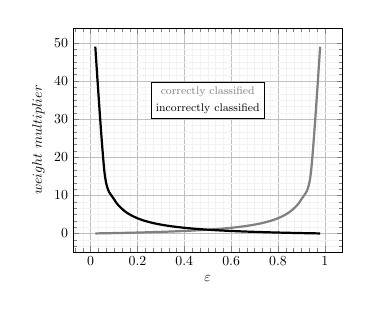
\begin{tikzpicture}[
		scale=0.5
	]

		\begin{axis}[
			domain=0.02:0.98,
			minor tick num=5,
			grid=both,
    			grid style={line width=.1pt, draw=gray!10},
    			major grid style={line width=.2pt,draw=gray!50},
			legend pos=outer north east,
			xlabel={$\varepsilon$},
			ylabel={$weight\ multiplier$}
		]
    			\addplot[no marks,ultra thick,smooth,gray]{exp(-(ln((1-x)/x)))};
			\addplot[no marks,ultra thick,smooth,black]{exp(ln((1-x)/x))};

			\node[align=center,fill=white,draw=black] at (axis cs:0.5,35) {\textcolor{gray}{
				\footnotesize{correctly classified}}\\ \footnotesize{incorrectly classified}
			};
    		\end{axis}
		
	\end{tikzpicture}
\end{figure}
	}
	
	\footnotesize
	\begin{itemize}
		\item Classifier weights $\alpha_u$ grow exponentially
		\item Classifier weight is 0 if error is $\nicefrac{1}{2}$ (model cannot be trusted, random guessing)
		\item For high errors \highlight{$\Rightarrow$ Do the opposite of what the classifiers predicts}
	\end{itemize}
\end{frame}


% AdaBoost: Two Classes
\begin{frame}{AdaBoost: Two Classes}{}
	\begin{itemize}
		\item With two classes, $\textbf{-1}$ and \textbf{+1}, the final classifier $C^*$ can be written as:
		\begin{equation}
			H(\bm{x}) = sign \left( \sum_{u=1}^k \alpha_u h_u(\bm{x}) \right)
		\end{equation}
		\item $\alpha_u$ is defined as above
		\item The weight update for the examples is given by:
		\begin{equation}
			w_i^{new} = \frac{w_i^{old} \cdot \exp \{ -\alpha_u y^{(i)} h_i(\bm{x}^{(i)}) \}}{\sum_{i=1}^n w_i}
		\end{equation}
	\end{itemize}
\end{frame}


% Boosting Example
\begin{frame}{Boosting Example}{}
	\begin{itemize}
		\item Ensemble of \highlight{decision stumps} ($\widehat{=}$ tree with a single split only)
		\item 10 examples (5 from class \textbf{+1} and 5 from class \textbf{-1})
		\item Each example is initially weighted with a factor of $\nicefrac{1}{10}$
	\end{itemize}

	\begin{figure}
		\includegraphics[scale=0.50]{08_decision_trees/02_img/boosting_example}
	\end{figure}
\end{frame}


% Boosting Example (Ctd.) -- 1st Iteration
\begin{frame}{Boosting Example (Ctd.)}{$1^{st}$ Iteration}
	\begin{figure}
		\includegraphics[scale=0.60]{08_decision_trees/02_img/boosting_first_iteration}
	\end{figure}
\end{frame}


% Boosting Example (Ctd.) -- 2nd Iteration
\begin{frame}{Boosting Example (Ctd.)}{$2^{nd}$ Iteration}
	\begin{figure}
		\includegraphics[scale=0.60]{08_decision_trees/02_img/boosting_second_iteration}
	\end{figure}
\end{frame}


% Boosting Example (Ctd.) -- 3rd Iteration
\begin{frame}{Boosting Example (Ctd.)}{$3^{rd}$ Iteration}
	\begin{figure}
		\includegraphics[scale=0.60]{08_decision_trees/02_img/boosting_third_iteration}
	\end{figure}
\end{frame}


% Boosting Example (Ctd.)
\begin{frame}{Boosting Example (Ctd.)}{Prediction}
	\vspace*{-2mm}
	\begin{figure}
		\includegraphics[scale=0.45]{08_decision_trees/02_img/boosting_prediction}
	\end{figure}
\end{frame}


% Subsection: Stacking
% --------------------------------------------------------------------------------------------------------
\subsection{Stacking}

% Combining Predictions
\begin{frame}{Combining Predictions}{}
	\begin{enumerate}
		\item \highlight{Voting} \checkmark
		\begin{itemize}
			\item Each classifier votes for one of the classes
			\item Each classifier has the same (model) weight
			\item This is \textbf{Bagging}
		\end{itemize}
		\item \highlight{Weighted Voting} \checkmark
		\begin{itemize}
			\item Weight the individual predictions with model weight
			\item This is \textbf{Boosting}
		\end{itemize}
		\item \highlight{Stacking}
		\begin{itemize}
			\item Use a \textbf{meta classifier} to combine the predictions
			\item See next slides...
		\end{itemize}
	\end{enumerate}
\end{frame}


% Stacking Algorithm
\begin{frame}[plain]{}{}
	\begin{algorithm}[H]
	\setstretch{1.3}
	\DontPrintSemicolon
	\footnotesize
	\KwIn{Training set $\mathcal{D}$, number of base classifiers $k$}
	Train $k$ base classifiers $C_1, C_2, \dots, C_k$\;
	Let all base classifiers predict the labels for the training set\;
	Create the meta data set (*)\;
	Train a meta classifier $M$ on the meta data set\;
 	\caption{Stacking Algorithm}
\end{algorithm}
	
	\vspace*{5mm}
	\footnotesize
	(*) Meta data set:\;
	\begin{itemize}
		\item \textbf{Labels}: \\
			Use the same labels as in the original data set
		\item \textbf{Attributes}: \\
			One attribute for each base classifier ($k$ attributes) \\
			The attribute values are the predictions of the corresponding classifiers
	\end{itemize}
\end{frame}


% Stacking Example
\begin{frame}{Stacking Example}{}
	\divideTwo{0.49}{
		\vspace*{2mm}
		\begin{table}[h]
	\scalebox{0.75}{
		\begin{tabular}{| c  c  c | c |}
			\hline
			\multicolumn{3}{| c |}{$\bm{Attributes}$}	&
			$\bm{Class}$
			\\ \hline
			$x^{(1)}_{1}$	&	$\dots$	&	$x^{(1)}_{m}$	&	$true$	\\
			$x^{(2)}_{1}$	&	$\dots$	&	$x^{(2)}_{m}$	&	$false$	\\
			$\dots$		&	$\dots$	&	$\dots$		&	$\dots$	\\
			$x^{(n)}_{1}$	&	$\dots$	&	$x^{(n)}_{m}$	&	$true$	\\ \hline
		\end{tabular}
	}
	\caption{Original training set}
\end{table}
	}{0.49}{
		\vspace*{1mm}
		\begin{table}[h]
	\scalebox{0.75}{
		\begin{tabular}{| c  c  c  c |}
			\hline
			$\bm{C_1}$	&
			$\bm{C_2}$	&
			$\dots$		&
			$\bm{C_k}$
			\\ \hline
			$true$	&	$true$	&	$\dots$	&	$false$	\\
			$false$	&	$true$	&	$\dots$	&	$true$	\\
			$\dots$	&	$\dots$	&	$\dots$	&	$\dots$	\\
			$false$	&	$false$	&	$\dots$	&	$true$	\\ \hline
		\end{tabular}
	}
	\caption{Predictions base classifiers}
\end{table}
	}
	\vspace*{-6mm}
	\begin{table}[h]
	\scalebox{0.75}{
		\begin{tabular}{| c  c  c  c | c |}
			\hline
			$\bm{C_1}$	&
			$\bm{C_2}$	&
			$\dots$		&
			$\bm{C_k}$	&
			$\bm{Class}$
			\\ \hline
			$true$	&	$true$	&	$\dots$	&	$false$	&	$true$	\\
			$false$	&	$true$	&	$\dots$	&	$true$	&	$false$	\\
			$\dots$	&	$\dots$	&	$\dots$	&	$\dots$	&	$\dots$	\\
			$false$	&	$false$	&	$\dots$	&	$true$	&	$true$	\\ \hline
		\end{tabular}
	}
	\caption{Meta data set}
\end{table}
\end{frame}


% Subsection: Error-correcting Output Codes
% --------------------------------------------------------------------------------------------------------
\subsection{Error-correcting Output Codes}

% Multi-Class-Problems
\begin{frame}{Multi-Class-Problems}{}\optional
	\begin{itemize}
		\item Usually, a \textbf{class binarization} technique is needed
		\item One-vs-Rest (one classifier for each class)
		\item Each class is encoded in a \textbf{bit-string}
	\end{itemize}
	
	\vspace*{3mm}
	\divideTwo{0.49}{
		\vspace*{4mm}
		\begin{table}[h]
	\scalebox{0.9}{
		\begin{tabular}{| c | c  c  c  c |}
			\hline
			\textbf{Class} & \multicolumn{4}{ c |}{\textbf{Class Vector}} \\ \hline
			a 	&	1	& 	0	&	0	&	0 \\ \hline	
			b 	&	0	& 	1	&	0	&	0 \\ \hline
			c 	&	0	& 	0	&	1	&	0 \\ \hline
			d 	&	0	& 	0	&	0	&	1 \\ \hline
		\end{tabular}
	}
\end{table}
	}{0.49}{
		\footnotesize
		\begin{boxBlueNoFrame}
			What would you do if the result were \textbf{1100}?
			It is not clear if the new instance belongs to class \textbf{a}
			or class \textbf{b}. \\
			\highlight{Solution: Use error-correcting output codes instead!}
		\end{boxBlueNoFrame}
	}
\end{frame}


% Error-Correcting Output Codes (ECOCs)
\begin{frame}{Error-Correcting Output Codes (ECOCs)}{}\optional
	\begin{itemize}
		\item Use code words that have a high pairwise \highlight{Hamming distance} $d$
		\item Can correct up to $(d - 1) / 2$ single bit-errors
		\item In this case: Use seven classifiers
		\begin{table}[h]
	\scalebox{0.7}{
		\begin{tabular}{| c | c  c  c  c  c  c  c |}
			\hline
			\textbf{Class} & \multicolumn{7}{ c |}{\textbf{Class Vector}} \\ \hline
			a 	&	1	& 	1	&	1	&	1	&	1	&	1	&	1 \\ \hline
			b 	&	0	& 	0	&	0	&	0	&	1	&	1	&	1 \\ \hline
			c 	&	0	& 	0	&	1	&	1	&	0	&	0	&	1 \\ \hline
			d 	&	0	& 	1	&	0	&	1	&	0	&	1	&	0 \\ \hline
		\end{tabular}
	}
\end{table}
		\item Predicted code-word: \textbf{1011111} $\Rightarrow$ What is the true class??? \\
			\textit{Probably class \textbf{a}, the second classifier made a mistake...}
	\end{itemize}
\end{frame}


% ECOCs: How to encode the classes?
\begin{frame}{ECOCs: How to encode the classes?}{}\optional
	\divideTwo{0.15}{
		\vspace*{5mm}
		\fbox{\includegraphics[scale=0.60]{08_decision_trees/02_img/binary}}
	}{0.84}{
		\begin{itemize}
			\item Criteria for the code words
			\begin{itemize}
				\item \textbf{Row separation} guarantees that errors can be corrected
				\item \textbf{Column separation}
					(identical columns $\Rightarrow$ Classifier makes same error several times)
			\end{itemize}
			\item \highlight{Exhaustive Codes}
			\begin{itemize}
				\item \textbf{Class 1:} Code word consists of 1s only
				\item \textbf{Class 2:} $2^{k-2}$ 0s followed by $2^{k-2}-1$ 1s
					($k\ \widehat{=}$ \# classes)
				\item \textbf{Class i:} Alternating runs of $2^{k-i}$ 0s and 1s \\
					(Last run is one bit shorter than the others)
			\end{itemize}
		\end{itemize}
	}
\end{frame}


% Section: Wrap-Up
%______________________________________________________________________
\section{Wrap-Up}
\makedivider{Wrap-Up}

% Subsection: Summary
% --------------------------------------------------------------------------------------------------------
\subsection{Summary}

% Summary
\begin{frame}{Summary}{}
	\begin{itemize}
		\item \textbf{Decision trees:}
		\begin{itemize}
			\item The construction of decision trees is guided by an \textbf{impurity measure}, \\
				e.\,g. entropy or Gini
			\item Recursively select features which \textbf{maximize the information gain}
			\item Decision trees can handle \textbf{numeric attributes} and \textbf{continuous output}
		\end{itemize}
		\item \textbf{Ensembles:}
		\begin{itemize}
			\item \textbf{Bagging:} Sample diverse data sets from underlying data
			\item \textbf{Boosting:} Focus on instances misclassified by earlier classifiers
			\item \textbf{Stacking:} Learn a meta-classifier on top of base classifiers
			\item \textbf{Random forests} combine bagging with randomization
		\end{itemize}
	\end{itemize}
\end{frame}


% Subsection: Self-Test Questions
% --------------------------------------------------------------------------------------------------------
\subsection{Self-Test Questions}

% Self-Test Questions
\begin{frame}{Self-Test Questions}{}\important
	\begin{enumerate}
		\item What is an inductive bias? What is the inductive bias of decision trees?
		\item Explain what Occam's razor is.
		\item What does entropy measure? How do you compute the information gain?
		\item True or false: \textit{'Pure data sets have maximal entropy.'}
		\item What is the advantage of ensemble methods?
		\item What distinguishes bagging from boosting?
		\item Explain what a random forest does.
	\end{enumerate}
\end{frame}


% Subsection: Lecture Outlook
% --------------------------------------------------------------------------------------------------------
\subsection{Lecture Outlook}

\begin{frame}{What's next...?}{}
	\makeoverview{7}
\end{frame}


% Subsection: Recommended Literature and further Reading
% --------------------------------------------------------------------------------------------------------
\subsection{Recommended Literature and further Reading}

% Literature
%______________________________________________________________________
\begin{frame}[allowframebreaks]{Recommended Literature and further Reading}{}
	\footnotesize
	\begin{thebibliography}{2}
		\literature{book}{Hastie et al. 2008}{[1] The Elements of Statistical Learning}
			{Hastie et al. Springer. 2008.}{$\rightarrow$ \href{
				https://web.stanford.edu/~hastie/Papers/ESLII.pdf
			}{\linkstyle{Link}}, cf. chapters 8.7, 8.8, 9.2, 10.1}\\
		\literature{book}{Tom M. Mitchell 1997}{[2] Machine Learning}
			{Tom M. Mitchell. McGraw-Hill. 1997.}{$\rightarrow$ \href{
				https://www.cs.ubbcluj.ro/~gabis/ml/ml-books/McGrawHill\%20-\%20Machine\%20Learning\%20-Tom\%20Mitchell.pdf
			}{\linkstyle{Link}}, cf. chapter 3}\\
		\literature{online}{Dave Sotelo, Online Blog}{[3] Using Bagging and Boosting to Improve Classification Tree Accuracy}{Dave Sotelo, Online Blog}{$\rightarrow$ \href{https://towardsdatascience.com/using-bagging-and-boosting-to-improve-classification-tree-accuracy-6d3bb6c95e5b}{\linkstyle{Link}}}
		\literature{book}{Bishop.2006}{[4] Pattern Recognition and Machine Learning}
			{Christopher Bishop. Springer. 2006.}{$\rightarrow$ \href{
				http://users.isr.ist.utl.pt/~wurmd/Livros/school/Bishop\%20-\%20Pattern\%20Recognition\%20And\%20Machine\%20Learning\%20-\%20Springer\%20\%202006.pdf
			}{\linkstyle{Link}}, cf. chapter 14.3}
	\end{thebibliography}
\end{frame}


% Subsection: Meme of the Day
% --------------------------------------------------------------------------------------------------------
\subsection{Meme of the Day}

% Meme of the Day
\begin{frame}{Meme of the Day}{}
	\begin{figure}
		\includegraphics[scale=0.65]{08_decision_trees/02_img/meme_of_the_day}
	\end{figure}
\end{frame}


% Thank you
%______________________________________________________________________
\makethanks

\end{document}